\section{Project dependencies}

Before even downloading \ESCRIBA, you require from some additional tools. These
tools or dependencies are for code formatting of drawings compilation and
rendering. Some of those are optional, but it is recommended that you install
all of them.

The required dependencies by \ESCRIBA are:

\begin{itemize}
  \item \href{https://www.gnu.org/software/make/}{Make}: a tool for automating
        processes, originally designed for controlling the generation of
        executables and other non-source files. By making use of a Makefile,
        different rules are provided for managing all your \LaTeX project.
  \item \href{https://www.latex-project.org/}{\LaTeX}: of course, without it you
        will not be able to render any document.
  \item \href{https://www.ghostscript.com/}{Ghostscript (optional)}: used for building
        drawings created by the Asymptote software.
  \item \href{https://asymptote.sourceforge.io/}{Asymptote (optional)}: a framework which
        allows the creation of vectorial drawings by making use of custom
        scripts. It is a very powerful tool for drawing beautiful scientific
        figures which would be complex of getting if using
        \href{https://es.overleaf.com/learn/latex/TikZ_package}{TkiZ}.
  \item \href{https://www.python.org/}{Python}: because \ESCRIBA is a
        \href{https://github.com/cookiecutter/cookiecutter}{cookiecutter} template, you will need this programming
        language to create a new project.
\end{itemize}

From now on, it will be assumed that the operative system you are using is a
Linux based one, in particular the \href{https://ubuntu.com/download}{Ubuntu}
flavor. The only thing which differs from this flavor with the rest is the
package manager you use for installing the dependencies.

\subsection{Installing the dependencies}

For installing the different dependencies, use your favorite package manager. As
said before, Ubuntu is the Linux distribution being used as example. Therefore,
follow the command exposed by figure \ref{fig:install_deps}:

\begin{figure}[h]
  \centering
  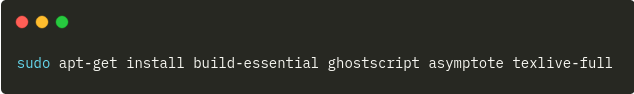
\includegraphics[width=\linewidth]{static/install_deps.png}
  \caption{The command to be used for installing the dependencies.}
  \label{fig:install_deps}
\end{figure}

Regarding Python installation, it is likely that your system already ships with
it. Nevertheless, you can download it from the official Python webpage. To do
so, use the link provided below these lines:

\begin{center}
  Download Python: \href{https://www.python.org/downloads/}{https://www.python.org/downloads/}
\end{center}

Once you have downloaded Python and installed it, it is time for installing the
\href{https://github.com/cookiecutter/cookiecutter}{cookiecutter} package. This
package allows for building templates, so you can start a new \ESCRIBA project
whenever you want. Run the same command from figure
\ref{fig:install_cookiecutter}:

\begin{figure}[h]
  \centering
  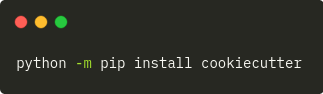
\includegraphics[scale=0.5]{static/install_cookiecutter.png}
  \caption{The command to install cookiecutter package.}
  \label{fig:install_cookiecutter}
\end{figure}
